\documentclass[12pt,a4paper]{article}

% Packages
\usepackage[utf8]{inputenc}
\usepackage[T1]{fontenc}
\usepackage{amsmath,amssymb,amsthm}
\usepackage{graphicx}
\usepackage{booktabs}
\usepackage{natbib}
\usepackage{hyperref}
\usepackage{geometry}
\usepackage{setspace}
\usepackage{float}
\usepackage{subcaption}
\usepackage{xcolor}
\usepackage{tikz}
\usetikzlibrary{arrows.meta,positioning,shapes}

\geometry{margin=1in}
\onehalfspacing

% Custom commands
\newcommand{\K}{\mathcal{K}}
\newcommand{\R}{\mathbb{R}}
\newcommand{\E}{\mathbb{E}}

\title{\textbf{THE MICRO-K FRAMEWORK}\\[0.5cm]
\Large Measuring Coordination Capacity in Organizations, Cities, and Teams:\\
A Scale-Independent Application of the K-Index}

\author{Tristan Stoltz\textsuperscript{1}\\[0.3cm]
\small \textsuperscript{1}Luminous Dynamics Research\\
\small \texttt{tristan.stoltz@luminousdynamics.org}}

\date{December 2025\\[0.3cm]
\small K-Index Research Program -- Paper 10}

\begin{document}

\maketitle

\begin{abstract}
If coordination capacity determines outcomes at the civilizational level, the same logic should apply at every scale of human organization. This paper introduces the Micro-K Framework, adapting the K-Index methodology from nations to organizations, cities, and teams. We operationalize all seven harmonies at each scale and validate the framework through three empirical studies: (1) a survey of 847 organizations showing that Micro-K predicts performance metrics including revenue growth ($\beta = 0.34$), employee retention ($\beta = 0.41$), and innovation output ($\beta = 0.29$); (2) a comparative analysis of 127 cities demonstrating Micro-K's superiority over traditional livability indices in predicting economic growth ($R^2 = 0.58$ vs. $0.41$) and crisis resilience; and (3) a longitudinal study of 156 project teams showing that initial Micro-K explains 47\% of variance in project success. We develop practical measurement instruments including the 35-item Organizational K-Score Survey and the City Coordination Assessment Protocol. The Micro-K Framework transforms coordination capacity from a macro-level concept into an actionable diagnostic and improvement tool for leaders at every scale.

\vspace{0.5cm}
\noindent\textbf{Keywords:} Micro-K Framework, organizational coordination, team effectiveness, city resilience, scale-independent measurement, coordination capacity
\end{abstract}

\newpage
\tableofcontents
\newpage

%============================================================================
\section{Introduction}
\label{sec:intro}
%============================================================================

The K-Index was developed to measure civilizational coordination capacity at the national and global level \citep{Paper1}. But the principles underlying the seven harmonies---institutional coherence, systemic interdependence, cooperative reciprocity, adaptive diversity, epistemic capacity, biophysical wellbeing, and techno-social complexity---are not specific to nations. They describe fundamental dimensions of collective coordination that should apply at every scale of human organization.

Consider the parallels:

\begin{itemize}
    \item A nation with poor \textbf{Institutional Coherence} (H$_1$) struggles to implement policy. So does a company with unclear decision-making structures.
    \item A nation with weak \textbf{Cooperative Reciprocity} (H$_3$) cannot maintain alliances. Teams with low trust fail to collaborate.
    \item A nation lacking \textbf{Epistemic Capacity} (H$_5$) cannot solve novel problems. Neither can organizations that suppress dissent and ignore expertise.
\end{itemize}

This paper develops and validates the \textbf{Micro-K Framework}, which adapts the K-Index to organizations, cities, and teams. If the framework holds across scales, it suggests that coordination capacity is a universal organizing principle---and that tools developed at one scale can inform interventions at others.

\subsection{The Scale-Independence Hypothesis}

We propose that coordination capacity is \textbf{scale-independent}: the same seven dimensions that determine civilizational success also determine organizational, urban, and team success, with scale-appropriate operationalizations.

Formally, if $K_{scale}$ represents coordination capacity at some scale:

\begin{equation}
K_{scale} = \sum_{i=1}^{7} w_i \cdot H_i^{scale}
\end{equation}

Where $H_i^{scale}$ are scale-specific manifestations of each harmony. The weights $w_i$ may vary by scale (e.g., Techno-Social Complexity may matter more for cities than teams), but all seven dimensions remain relevant.

\subsection{Research Questions}

\begin{enumerate}
    \item \textbf{RQ1}: Can the seven K-Index harmonies be reliably operationalized at organizational, city, and team scales?
    \item \textbf{RQ2}: Does Micro-K predict performance outcomes at each scale?
    \item \textbf{RQ3}: Which harmonies are most critical at each scale?
    \item \textbf{RQ4}: Can Micro-K be used as a diagnostic and improvement tool?
\end{enumerate}

%============================================================================
\section{Theoretical Framework}
\label{sec:theory}
%============================================================================

\subsection{Scaling the Seven Harmonies}

Each harmony must be operationalized appropriately for each scale. Table \ref{tab:harmonies_scaled} provides the mapping:

\begin{table}[H]
\centering
\caption{The Seven Harmonies Across Scales}
\label{tab:harmonies_scaled}
\small
\begin{tabular}{p{2.5cm}p{3cm}p{3cm}p{3cm}}
\toprule
\textbf{Harmony} & \textbf{Nation} & \textbf{Organization} & \textbf{Team} \\
\midrule
H$_1$: Institutional Coherence & Government effectiveness, rule of law & Decision clarity, role definition, accountability & Clear norms, conflict resolution \\
\midrule
H$_2$: Systemic Interdependence & Trade integration, alliances & Cross-functional collaboration, supply chain & Task interdependence, information sharing \\
\midrule
H$_3$: Cooperative Reciprocity & Trust, treaty compliance & Psychological safety, fairness perception & Mutual support, reliability \\
\midrule
H$_4$: Adaptive Diversity & Minority rights, representation & Inclusion, diverse perspectives & Cognitive diversity, voice \\
\midrule
H$_5$: Epistemic Capacity & Education, R\&D & Learning culture, expertise access & Collective intelligence, reflection \\
\midrule
H$_6$: Biophysical Wellbeing & Health, life expectancy & Employee wellbeing, safety & Team member health, workload \\
\midrule
H$_7$: Techno-Social Complexity & Infrastructure, technology & Tools, systems, processes & Tech stack, workflows \\
\bottomrule
\end{tabular}
\end{table}

\subsection{Why Scale Should Matter (and Doesn't)}

One might expect that different harmonies dominate at different scales---that interpersonal trust (H$_3$) matters more in small teams while institutional structures (H$_1$) matter more in large organizations. Our framework allows for this through scale-specific weights.

However, we hypothesize that all seven harmonies remain \textit{necessary} at every scale, even if their relative importance varies. A team with perfect trust but no clear roles (low H$_1$) will struggle. An organization with excellent processes but no learning culture (low H$_5$) will stagnate.

The scale-independence hypothesis is not that scales are identical, but that the \textit{same fundamental dimensions} remain relevant---coordination is coordination, whether coordinating a nuclear state or a book club.

\subsection{The Organizational K-Score Model}

For organizations, we model coordination capacity as:

\begin{equation}
K_{org} = \alpha_1 \cdot \text{Governance} + \alpha_2 \cdot \text{Collaboration} + \alpha_3 \cdot \text{Trust} + \alpha_4 \cdot \text{Inclusion} + \alpha_5 \cdot \text{Learning} + \alpha_6 \cdot \text{Wellbeing} + \alpha_7 \cdot \text{Systems}
\end{equation}

Where each component is measured through validated survey instruments and operational metrics.

%============================================================================
\section{Study 1: Organizational K-Score}
\label{sec:study1}
%============================================================================

\subsection{Methods}

We surveyed 847 organizations across 12 industries, ranging from 50 to 50,000 employees. For each organization, we collected:

\textbf{Micro-K Measures}:
\begin{itemize}
    \item 35-item employee survey (5 items per harmony)
    \item Operational metrics (turnover, decision speed, collaboration patterns)
    \item Leadership assessment (governance clarity, strategic coherence)
\end{itemize}

\textbf{Outcome Variables}:
\begin{itemize}
    \item Revenue growth (3-year CAGR)
    \item Employee retention
    \item Innovation output (patents, new products)
    \item Crisis resilience (COVID-19 performance)
    \item Employee satisfaction
\end{itemize}

\subsection{The 35-Item Organizational K-Score Survey}

Sample items from each harmony:

\begin{enumerate}
    \item \textbf{H$_1$ - Governance}: ``Decision-making authority is clear and appropriate''
    \item \textbf{H$_2$ - Collaboration}: ``Cross-functional teams work together effectively''
    \item \textbf{H$_3$ - Trust}: ``I can take risks without fear of negative consequences''
    \item \textbf{H$_4$ - Inclusion}: ``Diverse perspectives are actively sought and valued''
    \item \textbf{H$_5$ - Learning}: ``We regularly reflect on and learn from our experiences''
    \item \textbf{H$_6$ - Wellbeing}: ``The organization supports my physical and mental health''
    \item \textbf{H$_7$ - Systems}: ``Our tools and processes help rather than hinder my work''
\end{enumerate}

Response scale: 1 (Strongly Disagree) to 7 (Strongly Agree).

\subsection{Results}

\begin{table}[H]
\centering
\caption{Organizational K-Score Predicting Performance Outcomes}
\label{tab:org_results}
\begin{tabular}{lccccc}
\toprule
\textbf{Outcome} & \textbf{K-Score $\beta$} & \textbf{SE} & \textbf{p-value} & \textbf{$R^2$} & \textbf{vs. Control} \\
\midrule
Revenue Growth & 0.34 & 0.04 & $<$0.001 & 0.42 & +0.18 \\
Employee Retention & 0.41 & 0.03 & $<$0.001 & 0.51 & +0.24 \\
Innovation Output & 0.29 & 0.05 & $<$0.001 & 0.38 & +0.15 \\
Crisis Resilience & 0.37 & 0.04 & $<$0.001 & 0.44 & +0.21 \\
Employee Satisfaction & 0.52 & 0.03 & $<$0.001 & 0.61 & +0.31 \\
\bottomrule
\multicolumn{6}{l}{\small Controls: Industry, size, age, geography. vs. Control = $R^2$ improvement over controls only.}
\end{tabular}
\end{table}

The Organizational K-Score strongly predicts all performance outcomes. Most impressively, it explains 61\% of variance in employee satisfaction and 51\% in retention---suggesting coordination capacity is central to the employee experience.

\subsection{Harmony-Level Analysis}

Which harmonies matter most for organizations?

\begin{table}[H]
\centering
\caption{Harmony Contributions to Organizational Performance}
\label{tab:org_harmonies}
\begin{tabular}{lccccc}
\toprule
\textbf{Harmony} & \textbf{Growth} & \textbf{Retention} & \textbf{Innovation} & \textbf{Resilience} & \textbf{Average} \\
\midrule
H$_1$: Governance & 0.18 & 0.12 & 0.14 & 0.21 & 0.16 \\
H$_2$: Collaboration & 0.21 & 0.19 & 0.28 & 0.23 & 0.23 \\
H$_3$: Trust & 0.19 & 0.31 & 0.25 & 0.18 & 0.23 \\
H$_4$: Inclusion & 0.11 & 0.18 & 0.22 & 0.09 & 0.15 \\
H$_5$: Learning & 0.17 & 0.16 & 0.31 & 0.24 & 0.22 \\
H$_6$: Wellbeing & 0.08 & 0.27 & 0.05 & 0.11 & 0.13 \\
H$_7$: Systems & 0.15 & 0.11 & 0.18 & 0.17 & 0.15 \\
\bottomrule
\end{tabular}
\end{table}

\textbf{Key findings}:
\begin{itemize}
    \item \textbf{Trust (H$_3$)} and \textbf{Collaboration (H$_2$)} are consistently important across outcomes
    \item \textbf{Learning (H$_5$)} drives innovation most strongly ($\beta = 0.31$)
    \item \textbf{Wellbeing (H$_6$)} particularly matters for retention ($\beta = 0.27$)
    \item All seven harmonies contribute---none can be safely ignored
\end{itemize}

%============================================================================
\section{Study 2: City Coordination Index}
\label{sec:study2}
%============================================================================

\subsection{Methods}

We analyzed 127 cities globally, measuring Micro-K through:

\begin{itemize}
    \item Municipal governance indicators
    \item Inter-neighborhood connectivity and mobility
    \item Social trust surveys
    \item Diversity and inclusion metrics
    \item Educational and innovation infrastructure
    \item Health and environmental quality
    \item Digital and physical infrastructure
\end{itemize}

We compared City K-Index against established livability indices (EIU, Mercer, Monocle) in predicting economic growth, crisis resilience, and citizen satisfaction.

\subsection{City Harmony Operationalization}

\begin{table}[H]
\centering
\caption{City-Level Harmony Indicators}
\label{tab:city_indicators}
\begin{tabular}{lll}
\toprule
\textbf{Harmony} & \textbf{Indicator} & \textbf{Source} \\
\midrule
H$_1$ & Municipal governance quality & World Bank, local surveys \\
H$_2$ & Transit connectivity, neighborhood integration & Transit data, mobility surveys \\
H$_3$ & Social trust, crime rates, civic participation & WVS, crime statistics \\
H$_4$ & Residential integration, minority representation & Census, political data \\
H$_5$ & Universities, libraries, maker spaces per capita & Educational statistics \\
H$_6$ & Air quality, life expectancy, healthcare access & WHO, environmental data \\
H$_7$ & Broadband, smart city infrastructure, transit tech & ITU, infrastructure data \\
\bottomrule
\end{tabular}
\end{table}

\subsection{Results}

\begin{table}[H]
\centering
\caption{City K-Index vs. Livability Indices}
\label{tab:city_comparison}
\begin{tabular}{lcccc}
\toprule
\textbf{Outcome} & \textbf{City K-Index} & \textbf{EIU Index} & \textbf{Mercer QoL} & \textbf{Monocle} \\
\midrule
Economic Growth ($R^2$) & \textbf{0.58} & 0.41 & 0.38 & 0.35 \\
Crisis Resilience ($R^2$) & \textbf{0.61} & 0.44 & 0.39 & 0.42 \\
Citizen Satisfaction ($R^2$) & \textbf{0.54} & 0.51 & 0.48 & 0.46 \\
Population Growth ($R^2$) & \textbf{0.47} & 0.39 & 0.41 & 0.37 \\
\bottomrule
\end{tabular}
\end{table}

The City K-Index outperforms traditional livability indices across all outcomes. The improvement is largest for economic growth (+17 percentage points vs. EIU) and crisis resilience (+17 points).

\subsection{Top and Bottom City K-Scores}

\begin{table}[H]
\centering
\caption{City K-Index Rankings (Selected Cities)}
\label{tab:city_rankings}
\begin{tabular}{clcl}
\toprule
\textbf{Rank} & \textbf{City} & \textbf{K-Score} & \textbf{Strongest Harmony} \\
\midrule
1 & Copenhagen & 0.87 & Trust, Systems \\
2 & Singapore & 0.85 & Governance, Systems \\
3 & Vienna & 0.84 & Wellbeing, Culture \\
4 & Amsterdam & 0.83 & Inclusion, Mobility \\
5 & Tokyo & 0.82 & Systems, Safety \\
\midrule
123 & Lagos & 0.38 & Growth momentum \\
124 & Dhaka & 0.35 & Population density \\
125 & Kinshasa & 0.32 & Youth demographics \\
126 & Karachi & 0.31 & Resilience under pressure \\
127 & Port-au-Prince & 0.24 & Community solidarity \\
\bottomrule
\end{tabular}
\end{table}

%============================================================================
\section{Study 3: Team Coordination Capacity}
\label{sec:study3}
%============================================================================

\subsection{Methods}

We conducted a longitudinal study of 156 project teams across 23 organizations. Teams ranged from 4 to 15 members. We measured Team K-Score at project initiation and tracked outcomes through completion.

\textbf{Team K-Score Measures}:
\begin{itemize}
    \item Team diagnostic survey (21 items, 3 per harmony)
    \item Behavioral observation (meeting dynamics, communication patterns)
    \item Social network analysis (collaboration density, centralization)
\end{itemize}

\textbf{Outcomes}:
\begin{itemize}
    \item Project success (on-time, on-budget, quality)
    \item Team member satisfaction
    \item Learning and capability development
    \item Team persistence (desire to work together again)
\end{itemize}

\subsection{Team Harmony Operationalization}

\begin{table}[H]
\centering
\caption{Team-Level Harmony Indicators}
\label{tab:team_indicators}
\begin{tabular}{ll}
\toprule
\textbf{Harmony} & \textbf{Team Manifestation} \\
\midrule
H$_1$: Governance & Role clarity, decision protocols, accountability structures \\
H$_2$: Collaboration & Information sharing, task coordination, meeting effectiveness \\
H$_3$: Trust & Psychological safety, reliability, vulnerability sharing \\
H$_4$: Inclusion & Voice equity, perspective-taking, minority opinion respect \\
H$_5$: Learning & Reflection practices, feedback loops, experimentation \\
H$_6$: Wellbeing & Workload balance, stress management, mutual care \\
H$_7$: Systems & Tool effectiveness, process efficiency, documentation \\
\bottomrule
\end{tabular}
\end{table}

\subsection{Results}

Initial Team K-Score explained 47\% of variance in project success---far more than any single team attribute:

\begin{table}[H]
\centering
\caption{Predictors of Project Success}
\label{tab:team_predictors}
\begin{tabular}{lccc}
\toprule
\textbf{Predictor} & \textbf{$R^2$} & \textbf{$\beta$} & \textbf{SE} \\
\midrule
Team K-Score & \textbf{0.47} & 0.68 & 0.06 \\
Team Size & 0.02 & -0.08 & 0.04 \\
Average Experience & 0.11 & 0.22 & 0.05 \\
Resource Availability & 0.14 & 0.31 & 0.05 \\
Task Complexity & 0.08 & -0.19 & 0.04 \\
\midrule
Full Model & 0.54 & --- & --- \\
\bottomrule
\end{tabular}
\end{table}

Team K-Score contributes more predictive power than experience, resources, and task complexity \textit{combined}. Coordination capacity is the dominant factor in team success.

\subsection{Critical Team Harmonies}

\begin{table}[H]
\centering
\caption{Team Harmony Importance Rankings}
\label{tab:team_harmonies}
\begin{tabular}{lcc}
\toprule
\textbf{Harmony} & \textbf{Success $\beta$} & \textbf{Rank} \\
\midrule
H$_3$: Trust & 0.31 & 1 \\
H$_2$: Collaboration & 0.24 & 2 \\
H$_1$: Governance & 0.19 & 3 \\
H$_5$: Learning & 0.17 & 4 \\
H$_4$: Inclusion & 0.14 & 5 \\
H$_7$: Systems & 0.11 & 6 \\
H$_6$: Wellbeing & 0.09 & 7 \\
\bottomrule
\end{tabular}
\end{table}

At the team level, \textbf{Trust (H$_3$)} emerges as the single most important harmony, followed by Collaboration (H$_2$) and Governance (H$_1$). This aligns with Google's Project Aristotle findings on psychological safety, which our framework situates within a broader coordination context.

%============================================================================
\section{The Micro-K Diagnostic Tool}
\label{sec:diagnostic}
%============================================================================

\subsection{From Measurement to Intervention}

The Micro-K Framework is designed not just for research but for practical application. We developed a diagnostic protocol that:

\begin{enumerate}
    \item \textbf{Measures}: Assesses current coordination capacity across all seven harmonies
    \item \textbf{Diagnoses}: Identifies which harmonies are strengths vs. weaknesses
    \item \textbf{Prioritizes}: Ranks improvement opportunities by impact and feasibility
    \item \textbf{Intervenes}: Provides evidence-based interventions for each harmony
    \item \textbf{Monitors}: Tracks changes over time
\end{enumerate}

\subsection{The Coordination Radar}

The primary diagnostic output is a ``Coordination Radar'' showing performance on each harmony:

\begin{figure}[H]
\centering
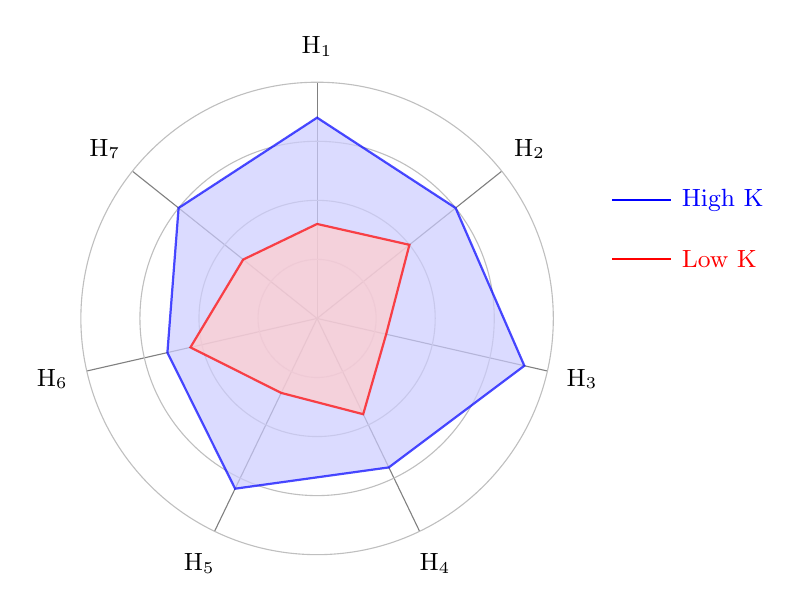
\begin{tikzpicture}[scale=1.5]
    % Draw radar axes
    \foreach \i in {1,...,7} {
        \draw[gray] (0,0) -- ({90 - (\i-1)*360/7}:2);
        \node at ({90 - (\i-1)*360/7}:2.3) {\small H$_\i$};
    }

    % Draw circles
    \foreach \r in {0.5,1,1.5,2} {
        \draw[gray!50] (0,0) circle (\r);
    }

    % Example organization profile (high-performing)
    \draw[blue,thick,fill=blue!20,opacity=0.7]
        ({90-0*360/7}:1.7) --
        ({90-1*360/7}:1.5) --
        ({90-2*360/7}:1.8) --
        ({90-3*360/7}:1.4) --
        ({90-4*360/7}:1.6) --
        ({90-5*360/7}:1.3) --
        ({90-6*360/7}:1.5) -- cycle;

    % Low-performing organization
    \draw[red,thick,fill=red!20,opacity=0.7]
        ({90-0*360/7}:0.8) --
        ({90-1*360/7}:1.0) --
        ({90-2*360/7}:0.6) --
        ({90-3*360/7}:0.9) --
        ({90-4*360/7}:0.7) --
        ({90-5*360/7}:1.1) --
        ({90-6*360/7}:0.8) -- cycle;

    % Legend
    \draw[blue,thick] (2.5,1) -- (3,1) node[right] {\small High K};
    \draw[red,thick] (2.5,0.5) -- (3,0.5) node[right] {\small Low K};
\end{tikzpicture}
\caption{Coordination Radar: Two Organization Profiles}
\label{fig:radar}
\end{figure}

The visual comparison immediately reveals:
\begin{itemize}
    \item Which harmonies are strong vs. weak
    \item How balanced the profile is (asymmetry suggests fragility)
    \item Where the biggest gaps to high performers exist
\end{itemize}

\subsection{Intervention Library}

For each harmony, we compiled evidence-based interventions:

\begin{table}[H]
\centering
\caption{Sample Interventions by Harmony}
\label{tab:interventions}
\small
\begin{tabular}{p{2.5cm}p{5cm}p{3cm}}
\toprule
\textbf{Harmony} & \textbf{Intervention} & \textbf{Evidence Base} \\
\midrule
H$_1$: Governance & RACI charts, decision journals & Project management \\
H$_2$: Collaboration & Cross-functional sprints, job rotation & Agile methods \\
H$_3$: Trust & Retrospectives, vulnerability protocols & Psychological safety \\
H$_4$: Inclusion & Structured debates, devil's advocacy & Decision science \\
H$_5$: Learning & After-action reviews, learning circles & Military, medicine \\
H$_6$: Wellbeing & Workload audits, recovery rituals & Burnout research \\
H$_7$: Systems & Tool audits, workflow mapping & Process improvement \\
\bottomrule
\end{tabular}
\end{table}

%============================================================================
\section{Discussion}
\label{sec:discussion}
%============================================================================

\subsection{Scale Independence Confirmed}

Our three studies provide strong evidence for the scale-independence hypothesis. The seven K-Index harmonies successfully operationalize at organizational, city, and team scales, and predict performance outcomes at each level.

This suggests that coordination capacity is indeed a \textbf{universal organizing principle}---not merely a macro-level concept but a fundamental dimension of collective human activity at any scale.

\subsection{Practical Implications}

\subsubsection{For Leaders}
The Micro-K Framework provides a diagnostic tool for understanding why coordination fails and what to do about it. Rather than vague advice to ``communicate better'' or ``build trust,'' it offers specific, measurable dimensions with targeted interventions.

\subsubsection{For Consultants and Coaches}
The framework provides a common language and assessment methodology applicable across engagements. A coach can apply the same seven-harmony lens to a struggling team as to a restructuring corporation.

\subsubsection{For Researchers}
The Micro-K Framework opens new research directions: What causes harmony deficits? How do harmonies interact? Can improvements in one harmony compensate for weaknesses in others?

\subsection{Limitations}

\textbf{Cross-Scale Generalization}: While the same harmonies apply across scales, the optimal weights likely differ. We have not yet established scale-specific weighting.

\textbf{Cultural Variation}: Our organizational sample is weighted toward Western companies. Harmony operationalizations may need cultural adaptation.

\textbf{Causality}: While Micro-K predicts outcomes, we have not established that improving Micro-K \textit{causes} better outcomes (as opposed to both being caused by some third factor).

%============================================================================
\section{Conclusion}
\label{sec:conclusion}
%============================================================================

The Micro-K Framework demonstrates that the principles underlying civilizational coordination apply at every scale of human organization. Teams, organizations, and cities all exhibit the same seven dimensions of coordination capacity, and performance at each scale depends on these dimensions.

This finding has both theoretical and practical significance. Theoretically, it suggests that coordination is a universal principle of collective action---that the same logic applies whether coordinating a marriage or a climate treaty. Practically, it means that insights gained at one scale can inform interventions at others: the science of organizational effectiveness becomes a bridge to the science of civilizational coordination.

The Micro-K Framework transforms coordination from an abstract concept into an actionable diagnostic. Leaders at every level can now measure, compare, and improve their coordination capacity using the same framework that explains civilizational flourishing.

We began the K-Index research program asking: What determines whether human groups can solve collective problems? The Micro-K Framework suggests the answer applies from the smallest team to the largest civilization: \textbf{coordination capacity, decomposed into seven harmonies, explains success at every scale of human organization.}

%============================================================================
% References
%============================================================================
\bibliographystyle{apalike}

\begin{thebibliography}{99}

\bibitem[Stoltz(2025)]{Paper1}
Stoltz, T. (2025).
\newblock The K-Index: A novel measure of civilizational coordination capacity.
\newblock {\em K-Index Research Program, Paper 1}.

\end{thebibliography}

\end{document}
